%%%%%%%%%%%%%%%%%%%%%%%%%%%%%%%%%%%%%%%%%%%%%%%%%%%%%%%%%%%%%%%%%%%%%
% Use the koma-script document style
\documentclass{scrbook}
%\KOMAoptions{twoside=false} % disable two-side formatting for scrbook
% alternatively, for shorter essay, use the following
% \documentclass{scrartcl}
%%%%%%%%%%%%%%%%%%%%%%%%%%%%%%%%%%%%%%%%%%%%%%%%%%%%%%%%%%%%%%%%%%%%%

%%%%%%%%%%%%%%%%%%%%%%%%%%%%%%%%%%%%%%%%%%%%%%%%%%%%%%%%%%%%%%%%%%%%%
% Useful packages
\usepackage{mathtools}
\usepackage{amssymb,bm,bbold}
\usepackage{enumerate}

\usepackage{hhline}
\usepackage{float}

% CSCI-265
\usepackage{tikz}
\usetikzlibrary{automata, positioning, arrows}


%=================================
% pre-defined theorem environments
\usepackage{amsthm}
\newtheorem{theorem}{Theorem}
\newtheorem{lemma}{Lemma}
\newtheorem{proposition}{Proposition}
\newtheorem{corollary}{Corollary}
\newtheorem{definition}{Definition}
\newtheorem*{remark}{Remark}
\newtheorem*{assumption}{Assumption}

%=================================
% useful commands
\DeclareMathOperator*{\argmin}{arg\,min}
\DeclareMathOperator*{\argmax}{arg\,max}
\DeclareMathOperator*{\supp}{supp}

\def\vec#1{{\ensuremath{\bm{{#1}}}}}
\def\mat#1{\vec{#1}}

%=================================
% convenient notations
\newcommand{\XX}{\mathbb{X}}
\newcommand{\RR}{\mathbb{R}}
\newcommand{\NN}{\mathbb{N}}
\newcommand{\QQ}{\mathbb{Q}}
\newcommand{\ZZ}{\mathbb{Z}}
\newcommand{\EE}{\mathbb{E}}
\newcommand{\PP}{\mathbb{P}}

\newcommand{\sL}{\mathcal{L}}
\newcommand{\sX}{\mathcal{X}}
\newcommand{\sY}{\mathcal{Y}}

\newcommand{\ind}{\mathbb{1}}

\newcommand{\kleene}{{}^\ast}

%%%%%%%%%%%%%%%%%%%%%%%%%%%%%%%%%%%%%%%%%%%%%%%%%%%%%%%%%%%%%%%%%%%%%
% Typography, change document font
\usepackage[tt=false, type1=true]{libertine}
\usepackage[varqu]{zi4}
\usepackage[libertine]{newtxmath}
\usepackage[T1]{fontenc}

\usepackage[protrusion=true,expansion=true]{microtype}

\author{Guy Matz}

\begin{document}
	
\tikzset{
	->, % makes the edges directed 
%		>='stealth', % makes the arrow heads bold 
	node distance=3cm, % specifies the minimum distance between two nodes. Change if necessary. 
	every state/.style={thick, fill=gray!10}, % sets the properties for each ’state’ node 
	initial text=$ $, % sets the text that appears on the start arrow 
}
	
\title{Title}
% \maketitle

% \tableofcontents
% 
% %\bibliography{bibfile}
% 
% \end{document}


\begin{enumerate}

\item \textbf{Convert the following $\epsilon$-NFA to a DFA:}


  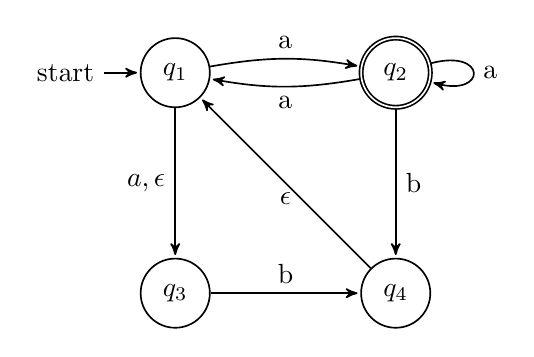
\begin{tikzpicture}[->,>=stealth',shorten >=1pt,auto,node distance=2.8cm,
  	semithick]
      \node[state, initial] (q1) {$q_1$};
      \node[state, accepting, right of=q1] (q2) {$q_2$};
      \node[state, below of=q1] (q3) {$q_3$};
      \node[state, right of=q3] (q4) {$q_4$};
      \draw 
    	(q2) edge[loop right] node{a} (q2)
      (q1) edge[bend left=10, above] node{a} (q2)
      (q2) edge[bend left=10,below] node{a} (q1)
      (q2) edge[right] node{b} (q4)
      (q3) edge[above] node{b} (q4)
            
      (q1) edge[left] node{$a, \epsilon$} (q3)
      (q4) edge[below] node{$\epsilon$} (q1)
      ;
  \end{tikzpicture}
\\\\

  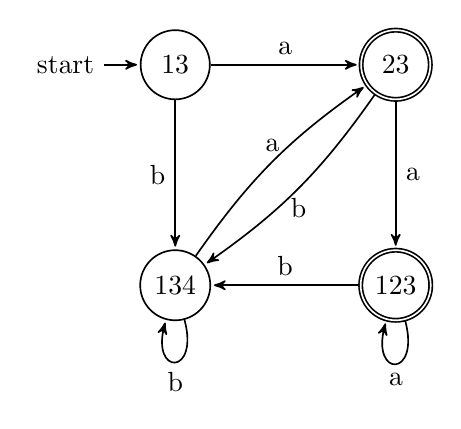
\begin{tikzpicture}[->,>=stealth',shorten >=1pt,auto,node distance=2.8cm,
  	semithick]
	\node[state, initial] (13) {13};
	\node[state, accepting,  right of=13] (23) {23};
	\node[state,  below of=13] (134) {134};
	\node[state, accepting,  below of=23] (123) {123};
	\draw
	(134) edge[loop below] node{b} (134)
	(123) edge[loop below] node{a} (123)	
	(13) edge[above] node{a} (23)
	(23) edge[right] node{a} (123)
	(13) edge[left] node{b} (134)
	(123) edge[above] node{b} (134)
	
	(23) edge[bend left=10, below] node{b} (134)
	(134) edge[bend left=10,above] node{a} (23)
	;
\end{tikzpicture}

\newpage
\item \textbf{Find a regular expression that describes the language accepted by the following $\epsilon$-NFA}
\begin{figure*}[h]
	
  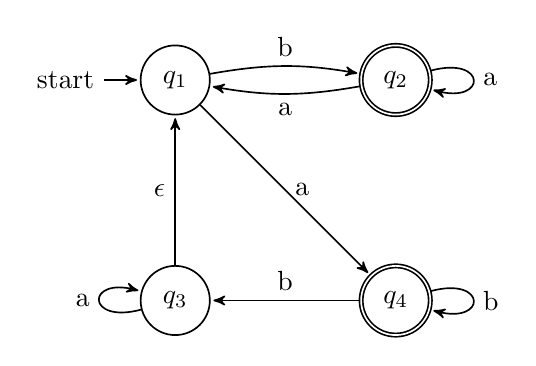
\begin{tikzpicture}[->,>=stealth',shorten >=1pt,auto,node distance=2.8cm,
  	semithick]
	\node[state, initial] (q1) {$q_1$};
	\node[state, accepting, right of=q1] (q2) {$q_2$};
	\node[state, below of=q1] (q3) {$q_3$};
	\node[state, accepting, right of=q3] (q4) {$q_4$};
	\draw
	(q2) edge[loop right] node{a} (q2)
	(q3) edge[loop left] node{a} (q3)
	(q4) edge[loop right] node{b} (q4)
	
	(q1) edge[bend left=10, above] node{b} (q2)
	(q2) edge[bend left=10,below] node{a} (q1)
	
	(q1) edge[right] node{a} (q4)
	(q4) edge[above] node{b} (q3)
	(q3) edge[left] node{$\epsilon$} (q1)
	;
\end{tikzpicture}

\end{figure*}
\\\\
$$(ba\kleene a + ab \kleene ba\kleene )\kleene (ba\kleene + ab\kleene)$$

\newpage
\item \textbf{Find the union and intersection of the 2 following DFAs:}
\\\\

  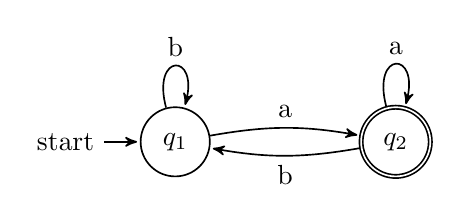
\begin{tikzpicture}[->,>=stealth',shorten >=1pt,auto,node distance=2.8cm,
  	semithick]
	\node[state, initial] (q1) {$q_1$};
	\node[state,  accepting, right of=q1] (q2) {$q_2$};
	\draw
	(q1) edge[loop above] node{b} (q1)
	
	(q1) edge[bend left=10,  above] node{a} (q2)
	(q2) edge[bend left=10, below] node{b} (q1)
	
	(q2) edge[loop above] node{a} (q2)
	;
\end{tikzpicture}

  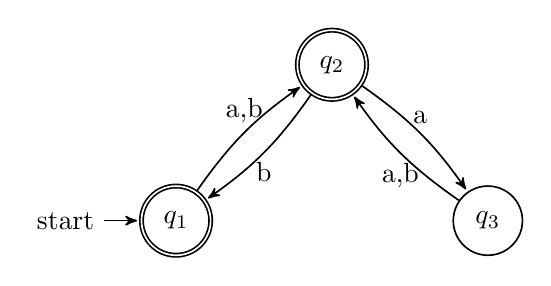
\begin{tikzpicture}[->,>=stealth',shorten >=1pt,auto,node distance=2.8cm,
  	semithick]
	\node[state, accepting, initial] (q1) {$q_1$};
	\node[state,  accepting, above right of=q1] (q2) {$q_2$};
	\node[state, below right of=q2] (q3) {$q_3$};
	\draw
	(q1) edge[bend left=10,  above] node{a,b} (q2)
(q2) edge[bend left=10, below] node{b} (q1)

	(q2) edge[bend left=10,  above] node{a} (q3)
(q3) edge[bend left=10, below] node{a,b} (q2)
	;
\end{tikzpicture}
\begin{enumerate}
	\item \textbf{Union:}
	
	  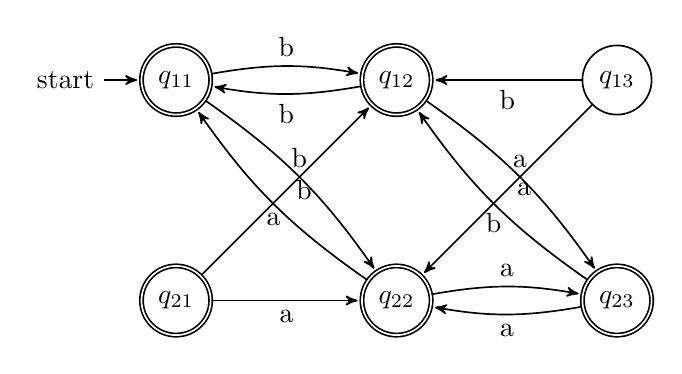
\begin{tikzpicture}[->,>=stealth',shorten >=1pt,auto,node distance=2.8cm,
	  	semithick]
		\node[state, accepting, initial] (q11) {$q_{11}$};
		\node[state,  accepting, right of=q11] (q12) {$q_{12}$};
		\node[state,  right of=q12] (q13) {$q_{13}$};
		\node[state, accepting, below of=q11] (q21) {$q_{21}$};
		\node[state,  accepting, right of=q21] (q22) {$q_{22}$};
		\node[state,  accepting, right of=q22] (q23) {$q_{23}$};
		
		\draw
		
		
		(q11) edge[bend left=10,  above] node{b} (q12)
		(q12) edge[bend left=10, below] node{b} (q11)
		
		(q13) edge[bend left=0, below] node{b} (q12)
		(q13) edge[bend left=0, right] node{a} (q22)

		(q21) edge[bend left=0, right] node{b} (q12)				
		(q21) edge[below] node{a} (q22)				
		(q22) edge[bend left=10,  above] node{a} (q23)
		(q23) edge[bend left=10, below] node{a} (q22)


(q12) edge[bend left=10,  above] node{a} (q23)
(q23) edge[bend left=10, below] node{b} (q12)
		
		(q11) edge[bend left=10,  above] node{b} (q22)
		(q22) edge[bend left=10, below] node{a} (q11)
		;
	\end{tikzpicture}
	
	\item \textbf{Intersection:}

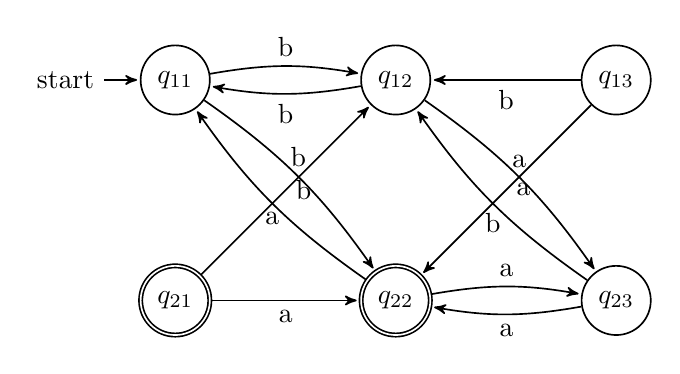
\begin{tikzpicture}[->,>=stealth',shorten >=1pt,auto,node distance=2.8cm,
	semithick]
	\node[state, initial] (q11) {$q_{11}$};
	\node[state,  right of=q11] (q12) {$q_{12}$};
	\node[state,  right of=q12] (q13) {$q_{13}$};
	\node[state, accepting, below of=q11] (q21) {$q_{21}$};
	\node[state,  accepting, right of=q21] (q22) {$q_{22}$};
	\node[state,  right of=q22] (q23) {$q_{23}$};
	
	\draw
	
	
	(q11) edge[bend left=10,  above] node{b} (q12)
	(q12) edge[bend left=10, below] node{b} (q11)
	
	(q13) edge[bend left=0, below] node{b} (q12)
	(q13) edge[bend left=0, right] node{a} (q22)
	
	(q21) edge[bend left=0, right] node{b} (q12)				
	(q21) edge[below] node{a} (q22)				
	(q22) edge[bend left=10,  above] node{a} (q23)
	(q23) edge[bend left=10, below] node{a} (q22)
	
	
	(q12) edge[bend left=10,  above] node{a} (q23)
	(q23) edge[bend left=10, below] node{b} (q12)
	
	(q11) edge[bend left=10,  above] node{b} (q22)
	(q22) edge[bend left=10, below] node{a} (q11)
	;
\end{tikzpicture}

\end{enumerate}

\newpage
\item \textbf{Draw a DFA that recognizes the language of all words where the number of a's is even or the total length of the word is divisible by 3.}
\\\\
Words in which the number of $a$'s is even:
\begin{figure*}[h]
	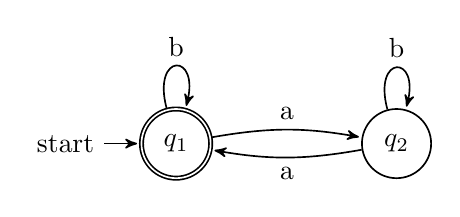
\begin{tikzpicture}[->,>=stealth',shorten >=1pt,auto,node distance=2.8cm,
		semithick]
		\node[state, accepting, initial] (q1) {$q_1$};
		\node[state,  right of=q1] (q2) {$q_2$};
		\draw
		(q1) edge[bend left=10,  above] node{a} (q2)
		(q2) edge[bend left=10, below] node{a} (q1)
		(q1) edge[loop above] node{b} (q1)
		(q2) edge[loop above] node{b} (q2)
		;
	\end{tikzpicture}
\end{figure*}
\\
Length of word is divisible by 3:
\begin{figure*}[h]
	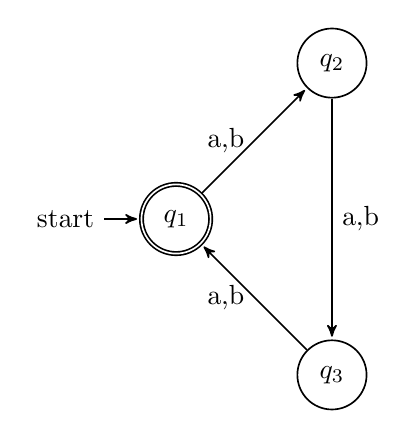
\begin{tikzpicture}[->,>=stealth',shorten >=1pt,auto,node distance=2.8cm,
	semithick]
	\node[state, accepting, initial] (q1) {$q_1$};
	\node[state,  above right of=q1] (q2) {$q_2$};
	\node[state, below right of=q1] (q3) {$q_3$};
	\draw
	(q1) edge[left] node{a,b} (q2)
	(q2) edge[right] node{a,b} (q3)
	(q3) edge[left] node{a,b} (q1)
	;
\end{tikzpicture}

\end{figure*}
\\

Union:  Words in which the number of $a$'s is even or the total length of the word is divisible by 3.
\begin{figure*}[h]
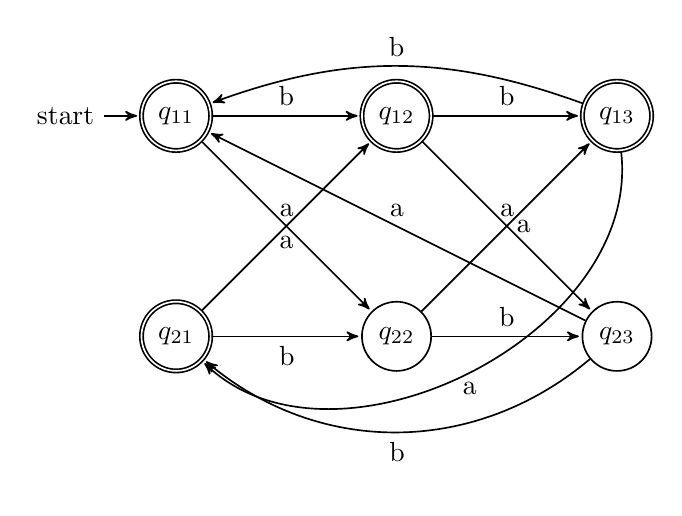
\begin{tikzpicture}[->,>=stealth',shorten >=1pt,auto,node distance=2.8cm,
	semithick]
	\node[state, accepting, initial] (q11) {$q_{11}$};
	\node[state, accepting,  right of=q11] (q12) {$q_{12}$};
	\node[state,  accepting, right of=q12] (q13) {$q_{13}$};
	\node[state, accepting, below of=q11] (q21) {$q_{21}$};
	\node[state,   right of=q21] (q22) {$q_{22}$};
	\node[state,  right of=q22] (q23) {$q_{23}$};
	
	\draw
	
	
	(q11) edge[above] node{b} (q12)
	(q12) edge[above] node{b} (q13)
	
	(q13) edge[bend right=20, above] node{b} (q11)
					
	(q21) edge[below] node{b} (q22)				
	(q22) edge[above] node{b} (q23)
	
	(q11) edge[above] node{a} (q22)
	(q21) edge[below] node{a} (q12)
	
	(q12) edge[above] node{a} (q23)
		(q23) edge[above] node{a} (q11)
	(q22) edge[right] node{a} (q13)
	
		(q13) edge[bend left=70, below] node{a} (q21)
		(q23) edge[bend left=40, below] node{b} (q21)
	;
\end{tikzpicture}
\end{figure*}

\newpage
\item \textbf{Try to turn the regular expression $(b+\epsilon) ab \kleene + (a+ \epsilon) ba \kleene$ into a DFA based on your intuition (like you would have on the first exam). Then, using the methods you've learned so far this semester, convert the regular expression first to an $\epsilon$-NFA (use Thompson's, but simplify the parts with clearly unnecessary $\epsilon$-transitions), then to a DFA, and then minimize it. Did you get the same answer? Can you learn anything about the regular expression from the minimized DFA that recognizes it?}
\\\\

??


\end{enumerate}

\input{footer.tex}
